%
% SUMMARY:
% USAGE:
%
% AUTHOR:       Christophe Prud'homme
% ORG:          Christophe Prud'homme
% E-MAIL:       prudhomm@zion
%
% ORIG-DATE:  7-Apr-04 at 16:48:32
% LAST-MOD:  7-Apr-04 at 23:07:19 by Christophe Prud'homme
%
% DESCRIPTION:
% DESCRIP-END.


%\documentclass[slidestop,compress,mathserif]{beamer}
\documentclass{article}
\usepackage[colorlinks=true]{hyperref}
\pdfinfo {
  /Title    (Presentation)
  /Author   (Christophe Prud'homme <christophe.prudhomme@imag.fr>)
  /Keywords   (Numerical Methods, Scientific Computing)
 }
\usepackage{fullpage}
\usepackage{multimedia,xmpmulti}
\usepackage[latin1]{inputenc}
\usepackage{graphicx}
\usepackage{float}
\usepackage{amsmath,amssymb}
\usepackage[noanswer]{exercise}
\usepackage{xcolor}
\definecolor{lbcolor}{rgb}{0.95,0.95,0.95}
\definecolor{cblue}{rgb}{0.,0.0,0.6}
\usepackage{filecontents,listings}


\lstset{language=c++,showspaces=false,showstringspaces=false,captionpos=t,literate={>>}{\ensuremath{>>}}1}
%\lstset{float}
\lstset{basicstyle=\small\ttfamily}
\lstset{lineskip=-2pt}
\lstset{keywordstyle=\color{red}\bfseries}
%\lstset{keywordstyle=\mdseries\color{red}}
\lstset{emph={inline},emphstyle=\color{red}\bfseries}
%\lstset{stringstyle=\ttfamily}
\lstset{commentstyle=\ttfamily\color{cblue}}
\lstset{backgroundcolor=\color{lbcolor},rulecolor=}
%\lstset{numbers=left}
%\lstset{numbers={none}}
%\lstset{numberstyle=\tiny}
%\lstset{numbersep=1pt}
\lstset{frame=single,framerule=0.5pt}
\lstset{belowskip=\smallskipamount}
\lstset{aboveskip=\smallskipamount}


\title{Calcul Scientifique en C++ et MPI}

\author{C. Prud'homme \& M. Ismail}
\date{UJF, 2008}

\begin{document}
\maketitle



\begin{Exercise}[title={p type Galerkin method in 1D}]
  \ExePart{Polynomials construction}

  \Question Plot the Legendre polynomials $(L_k)_{k=0...N}$ on
  $[-1;1]$ using for example octave up to order $10$. Save The values
  of the polynomials in a data file (e.g. \verb+'legendre.dat'+)
\begin{verbatim}
col1     col2  ...     col(11)
x_1  L_1(x_1)  ... L_{10}(x_1)
x_2  L_1(x_2)  ... L_{10}(x_2)
.           .                .
.           .                .
.           .                .
x_N  L_1(x_N)  ... L_{10}(x_N)
\end{verbatim}

  \Question Plot the Gauss points $(\xi^Q_q)_{q=0...Q}$ and weigths
  $(w^Q_q)_{q=0...Q}$. Verify numerically that they are indeed the roots
  of the Legendre polynomials (i.e. $L_k(\xi^{k-1}_i) = 0, i = 0,...,k-1$)

  \Question Now that we have constructed the Gauss points, they define
  a quadrature rule such that $(\xi^N_q,w^N_q)_{q=0...N}$ integrates
  exactly polynomials up to degree $2N+1$ (they are the roots of
  $P^{(0,0)}_{N+1}$). That is to say, if $p \in \mathbb{P}_{2N+1}(-1,1)$
  \begin{equation}
    \label{eq:1}
    \int_{-1}^1\ p(x)\ dx\ =\ \sum_{q=0}^{N}\ w_q\ p( \xi_q )
  \end{equation}
  \subQuestion Verify \eqref{eq:1} for $p(x)=x^5$.
  \subQuestion Verify that the Legendre polynomials are $L_2$ orthogonal.
  \begin{equation}
    \label{eq:3}
    \int_{-1}^1 L_i L_j = C_{ij} \delta_{ij}\ i,j=0...N
  \end{equation}
  \subQuestion Normalize them (e.g. $\|L_k\| = 1$ where $\|\cdot\|$ is the
  $L_2$ norm) and verify numerically that you have

  \begin{equation}
    \label{eq:2}
    \int_{-1}^1 L_i L_j =  \delta_{ij}\ i,j=0...N
  \end{equation}

  \ExePart
   Consider now a function $f$ (e.g. $f(x)=\exp(-x)$). We
  would like to construct its $L_2$ projection on
  $\mathbb{P}_N(-1,1)$, that is to say that we look for $p \in
  \mathbb{P}_N(-1,1)$ taking $(L_k)_{k=0...N}$ is used the basis spanning
  $\mathbb{P}_N(-1,1)$ such that
  \begin{equation}
    \label{eq:4}
    (p, L_k) = (f, L_k), \quad k=0...N
  \end{equation}
  Recall that
  \begin{equation}
    \label{eq:5}
    p=\sum_{i=0}^N\ p_i L_i.
  \end{equation}
  We have by pluging (\ref{eq:5}) into the system of relations~(\ref{eq:4})
  \begin{equation}
    \label{eq:6}
    \sum_{i=0}^N\ p_i (L_i,L_k) = (f, L_k)\quad k=0...N
  \end{equation}
  Since the $L_k$ are $L_2$ orthonormal(in other words the mass matrix
  $\int_{-1}^1 L_i L_k$ is the identity matrix), (\ref{eq:6}) becomes
  \begin{equation}
    \label{eq:7}
    p_k = (f, L_k)\ =\ \int_{-1}^1\ \exp(-x)\ L_k(x)\ dx, \quad k=0...N
  \end{equation}

  $(f,L_k), k=0...N$ is computed by using an appropriate quadrature
  rule (e.g Gauss)
  \begin{equation}
    \label{eq:8}
    \int_{-1}^1\ \exp(-x)\ L_k(x)\ dx \approx \sum_{q=0}^Q w_q\ \exp(-\xi_q)\ L_k(\xi_q)
  \end{equation}

  \Question Compute the components $(p_k)_{k=0}^N$ of $p$ in the basis
  $L_k$.
  \Question Compute $\|f-p\|=\sqrt{\int_{-1}^1 (f(x)-p(x))^2 dx}$ with $p$ its $L_2$ projection on
  $\mathbb{P}_N(-1,1)$ for $N=1,...,10$. Verify that
  \begin{equation}
    \label{eq:9}
    \|f-p\| \leq C 2^{-(N+1)}
  \end{equation}
  \Question Plot $f=\exp(-x)$
  on $[-1;1]$ and $p$ its $L_2$ projection on $\mathbb{P}_N(-1,1)$ for
  $N=1,...,10$

  \ExePart We now turn to the construction of other polynomials that
  we will express in the Legendre Basis. We consider only the Lagrange
  polynomials associated with the equisdistributed point set and the
  Gauss Lobatto point set.

  \Question Compute and compare the determinants of the Vandermonde
  matrix evaluated at equidistributed points and Gauss-Lobatto points
  associated to

  \subQuestion the canonical basis $(1, x, x^2, ...)$ from order 1 up to order 10
  \subQuestion the Legendre basis from order 1 up to order 10

  \Question Build the functional set and construct the Lagrange polynomials expressed in the Legendre basis
  \subQuestion associated to the equidistributed points on $[-1;1]$, $(h^e_k)_{k=0...N}$
  \subQuestion associated to the Gauss-Lobatto points on $[-1;1]$, $(h^{gl}_{k=0...N})$



  \Question Plot the Lagrange polynomials $(h^e_k)_{k=0...N}$ and $(h^{gl}_{k=0...N})$ up to $N=10$

  \ExePart
  We now turn to the resolution of the following 1D problem using a $p$ type Galerkin method: find $u$ such that
  \begin{equation}
    \label{eq:10}
    \begin{array}[c]{rl}
      -\Delta u &= f \text{ on } [-1;1]\\
      \displaystyle \frac{\partial u}{\partial n}(-1) &= e\\
      \displaystyle u(1) + \frac{\partial u}{\partial n}(1) &= 0\\
    \end{array}
  \end{equation}
  with $f(x)=\exp(-x)$.

  \Question Verify that $g=\exp(-x)$ is the solution  of \eqref{eq:10}.

  \Question Write the variational formulation and look for $u \in
  \mathbb{P}_N(-1,1)$ and take the test functions as a basis of
  $\mathbb{P}_N(-1,1)$ (e.g. Legendre)

  \Question Write the system in algebraic form
  \begin{equation}
    \label{eq:11}
    A \hat{u} = b
  \end{equation}
  where $\hat{u}$ are the components of $u$ in the basis of
  $\mathbb{P}_N(-1,1)$.
  You should get
  \begin{equation}
    \label{eq:12}
    \begin{array}[c]{rl}
      A_{ij} &= (\nabla \phi_i, \nabla \phi_j) - \phi_i(1)\phi_j(1)\\
      b_i &= (\phi_i,f) - e\ \phi_i(-1)
    \end{array}
  \end{equation}
  where $(\cdot,\cdot)$ still denote the $L_2$ scalar product.

  \Question Solve the system \eqref{eq:11} from order $N=1$ to $N=10$ for
  \subQuestion $(\phi_k = L_k)_{k=0...N}$ the Legendre polynomials
  \subQuestion $(\phi_k = h^{e}_k)_{k=0...N}$ the Lagrange polynomials at the equidistributed points on $[-1;1]$
  \subQuestion $(\phi_k = h^{gl}_k)_{k=0...N}$ the Lagrange polynomials at the Gauss Lobatto points on $[-1;1]$

  \Question Plot the solution in the previous cases up to order 10

  \Question Compute the $L_2$ norm of the error $\|g-u\|$ in the basis
  and verify that the $L_2$ norm behaves like an exponential with respect to $N$, i.e
  \begin{equation}
    \label{eq:13}
    \|g-u\| \leq C 2^{-(N+1)}
  \end{equation}
  where $C$ is a constant independant of $N$.
\end{Exercise}

\begin{Answer}
  \Question you can obtain \verb+'legendre.dat'+ thanks to
  \verb+'test_pset.cpp'+ file by choosing \verb+degree+ = 9
  (\verb+argv[1] = 9+ at running command).
Plotting \verb+'legendre.dat'+ with octave gives the figure \ref{fig:1}
\begin{figure}[H]
  \label{fig:1}
  \centering
  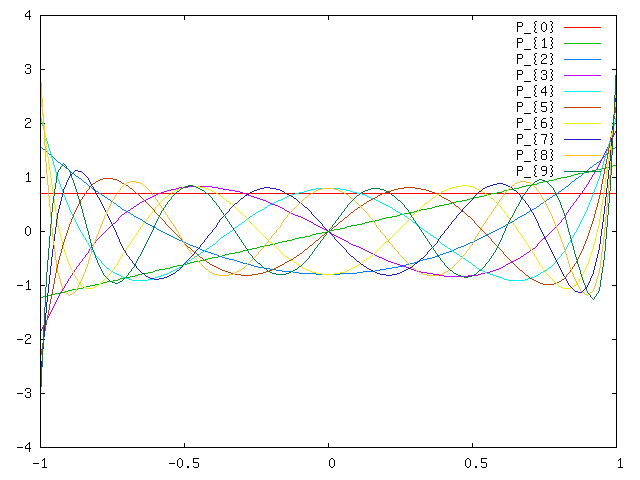
\includegraphics[scale=0.4]{legendre.png}
  \caption{Legendre polynomials $(L_k)_{k=0 \cdots 9}$}
\end{figure}

\end{Answer}

\end{document}


%%% Local Variables:
%%% mode: latex
%%% TeX-PDF-mode: t
%%% TeX-parse-self: t
%%% x-symbol-8bits: nil
%%% TeX-auto-regexp-list: TeX-auto-full-regexp-list
%%% TeX-master: t
%%% ispell-local-dictionary: "american"
%%% End:
